% \begin{savequote}[75mm]
% Nulla facilisi. In vel sem. Morbi id urna in diam dignissim feugiat. Proin molestie tortor eu velit. Aliquam erat volutpat. Nullam ultrices, diam tempus vulputate egestas, eros pede varius leo.
% \qauthor{Quoteauthor Lastname}
% \end{savequote}

\chapter{Interaction with Navigation Apps}
Previous works have so far focused on the experiences of drivers with early smartphone, dashboard-mounted and in-car GPS devices to aid in their navigation\cite{Brown2012TheGPS, Dingus1997a, Mahmud2009UserDrivers}. Here, I make a broader inquiry into the navigation practices of drivers who augment their driving with in-car navigation systems and or mobile applications. I also sought to understand the human factors behind their use of and compliance with the recommended optimal routes. In this qualitative descriptive study with 17 drivers, I recorded their commute and non-commute trips, and provide insights on how drivers engage with modern navigation systems, especially those that are infused with artificial intelligence from learned driving histories and crowd-sourced information. In this chapter, I:

\begin{enumerate}
\item illustrate how drivers integrate navigation systems and applications into their daily commute and non-commute trips;
\item describe if, when and where deviations from the recommended routes happen, as well as the reasons why certain navigating decisions are made;
\item discuss design implications for supporting the navigation needs of a driver; and 
\item reflect on how we can design better navigation experiences to support behavioral adaptation.
\end{enumerate}

\begin{table*}[t]
	\centering
    \caption{Participant demographic, socioeconomic and driving profiles. Legend: Fil - Filipino, Jap - Japanese, PHI - Philippines, JPN - Japan, CAN - Canada.}~\label{tab:s1-demographic}
    \begin{tabular}{l l l l l l l}
      & {\textbf{Driving}} & & & & {\textbf{Driving }}\\
      {\textbf{Participant}}
      & {\textbf{Years}}
      & {\textbf{Occupation}}
      & {\textbf{Nationality}} 
      & {\textbf{Domicile}}
      & {\textbf{Locations}}\\
      \hline
      P1 (F, 20) & 1-5 & Student & Fil & PHI & PHI \\
      P2 (M, 20) & 1-5 & Student & Fil & PHI & PHI \\
      P3 (M, 28) & 1-5 & IT Consultant & Fil & PHI & PHI \\
      P4 (M, 28) & 1-5 & Software Engineer & Fil & PHI & PHI \\
      P5 (F, 28) & 1-5 & Supervisor & Fil & CAN & CAN; USA\\
      P6 (M, 58) & $>$10 & Self-Employed & Fil & PHI & PHI \\
      P7 (M, 50) & $>$10 & Professor & Jap & JPN & JPN \\
      P8 (F, 28) & 1-5 & Nurse & Fil & PHI & PHI \\
      P9 (F, 28) & 1-5 & Consultant & Fil & PHI & PHI \\
      P10 (F, 28) & 1-5 & Medical Doctor & Fil & PHI & PHI \\
      P11 (M, 30) & 5-10 & Sales Director & Fil & PHI & PHI \\
      P12 (M, 20) & 1-5 & Student & Jap & JPN & JPN \\
      P13 (M, 20) & 1-5 & Student & Jap & JPN & JPN \\
      P14 (F, 42) & $>$10 & Pharmacy Assistant & Fil & JPN & JPN \\
      P15 (M, 29) & 1-5 & Entrepreneur & Fil & PHI & PHI \\
      P16 (M, 22) & 1-5 & IT Specialist & Fil & PHI & PHI \\
      P17 (M, 29) & 5-10 & Data Scientist & Fil & PHI & PHI \\
      \hline
    \end{tabular}
\end{table*}

\section{Participants} 
We recruited 17 driver participants with at least 1 year of driving experience and is using at least 1 navigation application or in-car navigation system through word-of-mouth and social network sharing (See Table \ref{tab:s1-demographic}). We only recruited drivers with at least a year of driving experience as they are likely to be adept in navigation and have acquired preferences (e.g. on safety, road condition, familiarity), but we did not recruit participants that involve driving as their main line of work (i.e. Uber drivers). We also made sure they are not novice users and currently using a navigation application or in-car navigation system as they are likely to have a considerable amount of experience with the features (e.g. turn-by-turn navigation, traffic condition, reporting). We recruited participants from Japan and the Philippines mainly because of their wide exposure to in-car navigation systems (in Japan) and navigation applications (in the Philippines). They also comprise an underrepresented driving population (Filipinos) in literature who may largely benefit from technology improvements. We aim to see common behaviors and factors considered despite the difference in driving culture and technologies used.  

Participants submitted their personal details (i.e. age, sex, occupation, and monthly income range) and driving background using a Google Form survey at the beginning. This allows for an examination of possible motivations for their commute and non-commute trips. We also asked whether they use in-car navigation systems and or navigation applications, and the number of years they have been using them. 

\section{Study Protocol}
After answering the pre-collection survey, we conducted a semi-structured qualitative study \cite{Soegaard2013} by recording trips in a naturalistic setup. Extending the scope of naturalistic driving data of Brown and Laurier \cite{Brown2012TheGPS} and Dingus et. al. \cite{Dingus1997a}, we focused on collecting data on the practices of using navigation applications for 3 trip types along with their trip context. We also collected data on whether they chose the recommendation or not, and the factors considered. Recordings were processed and trips were traced to extract instances of deviations. We then did a post-collection interview and used the grounded theory method \cite{Muller2016MachineMethod,Muller2014CuriosityMethod} for the survey answers, video recordings, trip data, in-car conversations and interviews to better understand their navigation practices and reason for route choices, and to uncover their motivations behind deviations made. 

\begin{figure*}[t]
  \centering
  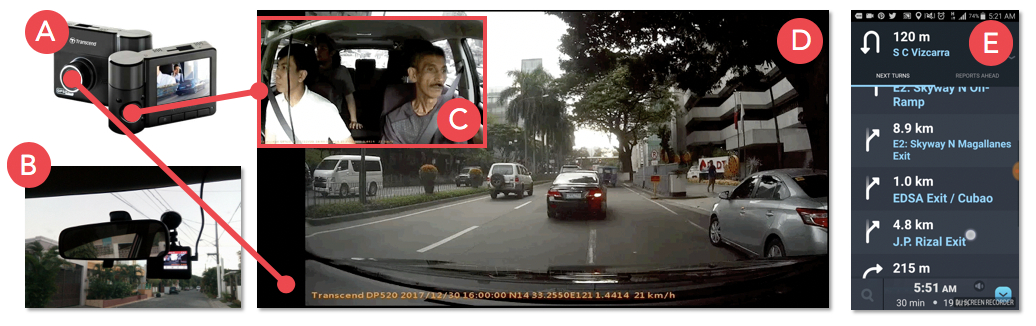
\includegraphics[scale=0.82]{figures/s1-data-collection-setup.png}
  \caption{The data collection setup. A) The commercial dash camera used; B) Position of the camera for optimal viewing angles; C) View of the driver and passengers; D) View of the road; E) Recording of the navigation application.}
  \label{fig:s1-setup}
\end{figure*}

\subsubsection{Trip Recordings}
Each participant were asked to record at least one instance of the following types of trips: Home-to-Work, Work-to-Home, and Home/Work-to-Unknown. The Home-to-Work and Work-to-Home trips represent their daily commutes. For the Home/Work-to-Unknown trips, the participants recorded their occasional trips to a location they do not usually go to or haven't been to before. 

Inside the participant's vehicles, we attached a commercial dual lens dash camera behind the rear-view mirror (Figure \ref{fig:s1-setup}B) to record the changing conditions on the road (Figure \ref{fig:s1-setup}D), and the driver and passenger/s attention (Figure \ref{fig:s1-setup}C). We wanted to capture how a driver and/or a navigator (because it can be someone besides the driver) behaves and what is seen on the road when a deviation happens. The dash camera also recorded the GPS tracks, speed, and in-car conversations. For P1, P2 and P6, a data collector was riding with them to perform shadowing and asked questions as needed. The rest of the participants collected by themselves and were asked to think aloud. Before each trip, participants noted down their origin, destination, reason for the trip or the first activity to be done upon arrival (e.g. attend a meeting, attend family gathering, etc.), and whether it was urgent. We were able to collect 65 trip recordings in total -- 18 work-to-home, 13 home-to-work, and 34 occasional non-commute trips. Among these, 12 trips did not have any deviations, leaving only 53 trips for analysis. 

\subsubsection{App Recordings}
To keep track of the application behavior and recommended routes, participants recorded the screen of their smartphones with the navigation application open (Figure \ref{fig:s1-setup}E). This allowed us to observe how the driver and/or navigator used the application while navigating. It also allows us to track how the application behaves after every deviation and how the driver adjusts to the changes.

\subsubsection{Trip Tracing and Processing}
After data collection, we viewed the trip and app recordings and manually traced each trip's actual route taken and the first recommended route using Google MyMaps. We then marked the deviations (if any) made, and the app's recommended rerouting after each deviation (Figure \ref{fig:s1-map-trace}). Trip durations and total distances of both actual and recommended routes were computed using the traces on Google MyMaps. We initially wanted to quantify gaze from the in-car videos but almost all drivers were using voice guidance. We did not pursue it but still observed where they paid attention to. 

\begin{figure*}[t]
  \centering
  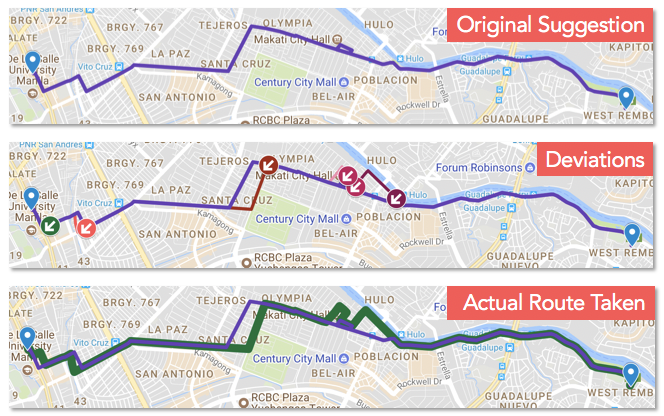
\includegraphics{figures/s1-map-tracing.png}
  \caption{Traces of the [Top] navigation application's recommendation in violet, [Middle] deviations made by the driver during the trip (arrows symbols), and [Bottom] the actual route taken by the driver in green.}
  \label{fig:s1-map-trace}
\end{figure*}

In preparation for the post-collection interviews, we synchronized the dash camera and app recordings, and made clippings that focused on parts of the trips when deviations happened. We included 10 seconds of video before and after each deviation to provide more context.

\subsubsection{Post-Collection Interview}
In a separate interview after the data collection and processing, we first asked the participants about their daily routines and their motivations and experiences in using navigation applications. We then presented their trip traces and synchronized clippings when deviations happened. The interviews lasted between 60 to 90 minutes on average, and were focused on recollecting navigation experiences and examining the motivations behind choosing a route, the deviations made(if any), perceptions about the road conditions and recommended routes, as well as other observations and insights from the videos. 

\subsubsection{Data Analysis}
Finally, we did an iterative coding and thematic analysis of the interview answers, in-car conversations and videos. We did a pilot analysis with 7 participants while the 10 other participants are still collecting. We achieved saturation after only a few new codes and themes were generated for the next 10 participants. In the following sections, I discuss the key findings of this qualitative descriptive study.

\section{Navigation Practices}
First, we want to investigate the applications used by the drivers, the information they sought, and the order by which the information were used. For this, we looked into the answers from the pre-collection questionnaire and compared it with the recordings and answers to the post-collection interview. We also used trip and app recordings to see associations with the type and purpose of trip. 

\subsection{Applications and systems used} 
In daily commute trips, Waze is primarily used when drivers have previous experiences of traffic congestion along their regular and familiar routes (H2W=66.7\%, W2H=69.2\%). They see Waze as an authoritative application especially when they have a clear intention to avoid being late or heavy traffic conditions. Even though Google Maps also provide turn-by-turn navigation and live/historical traffic information, drivers still put a lot of weight on the social aspect of Waze wherein other drivers can manually report traffic conditions, accidents, and road closures. Drivers gain a sense of confirmation as Waze shows manually reported traffic conditions to the ones they derive from the GPS tracks of connected drivers (P3, P4, P8). Since the road incident reports can be quite vague, drivers also acknowledge the usefulness of the public comment feature that allows other drivers who have passed by that area to share details about the incident. P6 shares that once when he was stuck near the tail of a standstill traffic, his passenger checked the public comments feature helped to get real-time updates from the drivers near an accident. It helped him decide whether he should wait longer or start finding other options. 

For short commute trips that doesn't have many alternative routes and doesn't normally experience significant traffic congestion, P5 opt to use Google Maps instead. She expects to see her regular route as the recommended route by the application and just checks the estimated time of arrival. Additionally, she shares that because Google Auto is installed in her vehicle, she prefers to use Google Maps because she can view the route guidance in a wider screen compared to her smartphone. 

Participants from Japan (P7, P12, P13, P14) were primarily using in-car navigation systems because of its ubiquity in most Japanese vehicles. Aside from the provided basic navigation features and digital maps, they are also connected to the local intelligent transportation systems. P13 shared that in one of his previous trips, his in-car navigation system provided a traffic advisory because of an accident in the national highway. It guided him to leave the national highway using the nearest exit.  

In places where the drivers in Japan (P7, P12, P13, P14) drove in, they did not experience any heavy traffic thus, they were not so compelled to download and use another navigation application. However in one of P14's recorded trips, she used and followed Waze when her in-car navigation system started giving incorrect directions. She was noticeably surprised when the in-car navigation system guided her to a direction that's opposite from the destination. She still made the turn as guided by the system but she had already asked one of the passengers to look for the next turn. The passenger then used Waze. P12 particularly used Waze in one of his occasional trips because it shows the location of speed cameras. He found it very useful especially when driving in an unfamiliar location. He shares that this is not provided by his in-car navigation system. 

Other than those mentioned above, drivers also sought information from social networking sites (e.g. Twitter and Facebook) to check traffic and incident updates from their friend networks and the pages of local transportation agencies (P3, P4, P6). They access these sources to augment the information that is not yet provided by in-car navigation systems and navigation applications. 

\subsection{Information Sought}

\begin{figure}[h]
  \centering
  \vspace{-.20cm}
  \centerline{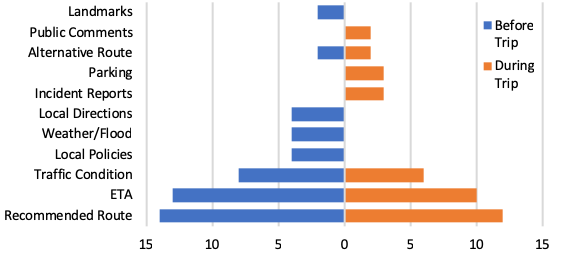
\includegraphics{figures/s1-info_sought.png}}
  \vspace{-.30cm}
  \caption{The number of participants who accessed certain types of information before and during their trips.}
  \label{fig:s1-info_sought}
\end{figure}

From the interviews and in-car conversations, we looked into the number of times that the participants mentioned each type of information as part of their trip planning and navigation (Figure~\ref{fig:s1-info_sought}). Three participants (age=28-29 y.o.) who have at least 5 years of continued application usage seek at most 7 of these, while the two youngest participants (age=20 y.o.) only check the ETA.

Drivers were mostly checking the estimated time of arrival of the recommended routes, the roads they needed to take, and the traffic condition as their main criteria for choosing a recommended route to follow. Some of the drivers also checked incident reports and updates (P4, P6) to know how much longer they needed to wait in congested roads. 

Drivers were also seeking localized and contextual information such as transport policies (e.g. travel demand management policies, truck ban hours) and flooding (P3, P4, P8). Common to Philippine metropolitan areas, travel demand management policies disallow certain vehicles to use public roads on specific time periods, and it can differ per city. P4 sought this information because he wants to know if he needs to leave earlier than usual to avoid getting apprehended or not use his car at all. Although some participants explicitly shared that they do not actually seek for this information anymore (i.e. P15, P16, P17) because they only memorized it once and doesn't change. However, we see this information useful for transport network vehicle (i.e. Uber, Lyft, Grab) drivers who take passengers to unknown destinations, across cities. In one instance shared by P6 as he was riding an Uber, the driver was apprehensive in crossing another city as recommended by his Waze application because the driver was not sure whether he's allowed or not. That city had a completely different travel demand management scheme as the rest of Metro Manila. Lastly, P7 shared that during winter, he is seeking local information about roads that are not too slippery and safe to drive on, especially because the main roads are where most cars will go. 

For longer and or occasional trips, drivers were also seeking information about familiar landmarks (P3, P4), good parking spaces and local directions. While in-car navigation systems and navigation applications can provide these information, drivers still seek the knowledge of a local person that knows the ins and outs of an unfamiliar place. 

\subsection{Usage behavior}
Drivers have been observed to have different behaviors in accessing information and using these to decide which route to take. 

Before starting their daily commute trips, drivers first check the estimated time of arrival (ETA) of the recommended route. They want to have a quick overview of how long it will take them to get to their destinations. Then, they check their familiarity with the roads that were recommended. They usually check how close it is to their regular routes. If it is completely new to the drivers, they check the alternative recommendations and see if their regular route is included. They check the differences between the estimated times of arrival and decide based on a criteria. If they are leaving very late and or in a rush, they only check the ETA (P4, P10). 

During the trip, drivers start the turn-by-turn navigation but only some of them chose to follow it. For example, P10 still follows her regular route to work but still keeps Waze on to get traffic updates. However in the case of P8, she shares that she always follows the suggested route.

When they suddenly experience slowing down due to unexpected traffic build up, they first check what caused it using the navigation application. If there are no reports on the application, they sometimes check Twitter and or Facebook (P3, P4). For alone drivers, they only get to check this information once they are slowing down or in a complete stop (P4, P17). But as passengers and navigators, they tend to check why there's a sudden slow down in traffic and try to look for possible alternative routes (i.e. P3, P4, P6, P16, P17).

For shorter trips to unknown locations, they only used one tool for route guidance. For longer trips, some participants use a mix of applications to plan and navigate. For instance, P3 and P4 shared that they use Google Maps for planning the trip and Waze during the actual trip. Using Google Maps, they looked for landmarks that they can use during the trip and familiarized themselves with the area. And then during the actual trip, they have Waze or Google Maps turned on from the beginning, but leave it idle. They would start to carefully listen to the directions when they already reach a point that they are unfamiliar with (i.e. P4, P15, P17). This supports Patel et. al.'s findings that drivers preferred routes that use familiar landmarks over very detailed turn-by-turn instructions \cite{Patel2006PersonalizingRoutes}. 

In some trips, they switched to another application because of unreliable or missing information. For example in P12's trip, they stopped following the in-car navigation because its map is not updated with the new roads. They then switched to Waze.

\section{Route Choice}

\begin{figure}[h]
  \centering
  \vspace{-0.10cm}
  \centerline{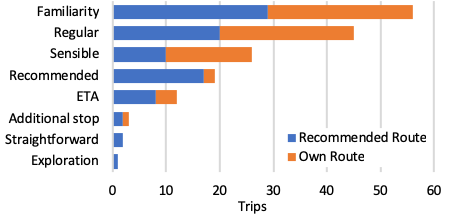
\includegraphics{figures/s1-reason_route_choice.png}}
  \vspace{-0.30cm}
  \caption{The factors considered for route choice and the number of trips that used them when they chose their own or a recommended route.}
  \label{fig:s1-reason_route_choice}
\end{figure}

We also wanted to investigate whether our participants chose to follow the recommended routes given by the applications and in-car navigation systems that they use. We used the app recordings to see how they engaged with an application before a trip. We checked if the destination and agenda upon arrival plays a role. We also analyzed what and how the descriptive and prescriptive information provided were used. 

After analyzing the trip recordings, we found our results consistent with the findings of Zhu and Levinson \cite{Zhu2015DoPrinciple}, and Tang et. al. \cite{Tang2016AnalyzingData}. Our 17 participants chose a route that is not the shortest nor fastest, as computed, in at least one of their recorded trips. At the beginning of each trip, participants decided to use their regular routes in 28 trips (43.1\%), where the occasional non-commute and home-to-work trips each comprised 42.9\%, and 14.3\% were work-to-home. On the other hand, 37 trips (56.9\%) decided to follow recommended routes at the beginning. Majority or 59.5\% of those trips were occasional non-commute, while the work-to-home and home-to-work trips comprised 24.3\% and 16.2\%, respectively. While this contrasts the low preference of drivers for fastest and shortest routes in Pfleging et. al.'s \cite{Pfleging2014ExperienceNavigation} study, this was mainly because Waze and Google Maps do not have options available for eco-routes while the in-car navigation systems used does not make that option apparent to the participants.

Figure~\ref{fig:s1-reason_route_choice} shows how many trips used a which factors to make a route choice decision. In majority or 65\% of the recorded trips, participants considered 3 factors, with familiarity as the most used factor. And while 56.9\% of trips used the recommendation at the beginning, only 21.6\% chose them because of fast ETA. This contrasts the high importance rating of the fastest route factor in the work of Pfleging et. al. \cite{Pfleging2014ExperienceNavigation}.

Before starting their daily commute trips, most participants checked the estimated time of arrival (ETA) and their familiarity with the roads in choosing a route to follow. When they had an important agenda (e.g. meetings, parties) and they were already running late, they chose the fastest recommendation of the application without consideration of familiarity (i.e. P4, P8). For P17, he always turns on the application and follows what recommendation is given. Sometimes, he would inspect the first few roads to decide otherwise.  

When some participants were leaving early and not in a hurry, they always compared the ETA of their regular route with the fastest recommendation. They would chose their regular routes over the fastest recommendation if the time difference is negligible. For instance, P15 shared that he would choose a new recommendation from Google Maps when it is at least 10 minutes faster. But when it is only 2-5 minutes faster, he would still choose a familiar or his regular route. Other participants shared that they would choose a recommended route as long as it has less traffic congestion (i.e. P3, P15), shorter distance (i.e. P3, P5) and straightforward paths (i.e. P8, P14). If some parts of the recommendations do not fit their criteria, they would make a decision to not follow it completely and rely on their own knowledge. 

For occasional non-commute trips, participants chose routes with familiar landmarks (P3, P4), roads familiar to them (P5, P6, P7), and routes suggested by friends living near their destination (P8, P9). For completely new destinations, most participants would follow the application or in-car navigation system completely.

Interestingly, some participants have other reasons for picking a route. For example, P6 shared the he once chose a route with a gas station along the way because they are taking a long trip while P14 chose a route with a specific restaurant along the way because they haven't eaten lunch yet. Other reasons include the need to visit convenience stores (P6, P7) and toilets (P13), and to drop off passengers on the way to work (P6).

Surprisingly, we also found that some participants will open their applications but choose not to follow whatever the application recommends, especially for commute trips. P9 shares that \emph{"In fact, I have self-awareness that in those moments that I know I can, I try to not [follow]."} She doesn't want to be too dependent on the application as she feels that \emph{"whenever there are cases that I cannot use it, I feel incapacitated."} Other participants like P6 shares that most of the time, he just takes his regular route and leave Waze on because he believes that it can learn his regular route. However, even after some months of doing so, the application still doesn't give his regular route as the first recommendation. This non-compliant and non-use behavior supports the findings of Al Mahmud et. al. that some drivers choose not to be too reliant on GPS devices because they know that it can make mistakes and they still have to make their own judgments \cite{Mahmud2009UserDrivers}. 

\section{Deviations}

\begin{figure}[h]
  \centering
  \vspace{-0.20cm}
  \centerline{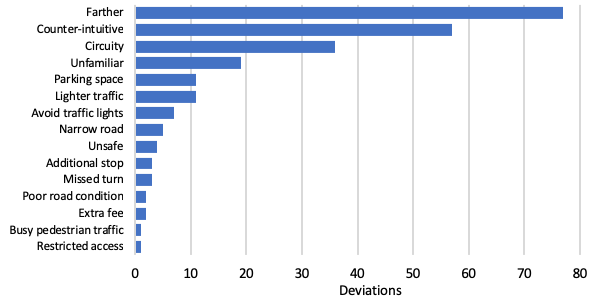
\includegraphics{figures/s1-reason_devs.png}}
  \vspace{-0.30cm}
  \caption{The factors for deviation and the number of deviations they caused.}
  \label{fig:s1-reason_devs}
\end{figure}

In understanding the motivations behind the deviations, we analyzed the videos, trip data and trip traces to see if any were deliberate or missed turns, and whether they were based on prior knowledge, on information from applications or situational awareness. During the 65 trips, participants deviated 153 times in total. They did it 39 times for home-to-work (M=2.17, SD=5.07), 30 times for work-to-home (M=2.31, SD=6.19), and 84 times for occasional non-commute trips (M=2.47, SD=1.65). 38.5\% of them were single deviations made near the beginning or end of trips, while the extreme cases (3.1\%) made 14-15 deviations. However, there is no clear connection between the types of trips and the number of deviations made. 

Comparing the estimated travel time of the recommended routes and the actual travel times, deviating at least once made the trips longer by an average of 3.11 minutes (N=53, SD=12.35). When only 1 deviation was made, travel times increased by an average of 0.13 minutes (N=25, SD=8.72), and 1.07 minutes (N=45, SD=10.24) for up to 4 deviations. In extreme cases of more than 5 deviations, an average increase of 14.63 minutes (N=8, SD=17.21) was experienced. Although none of the drivers perceived their trips to be longer nor farther after making deviations, this shows that travel time can get worse as more deviations are made.

Looking at trip purpose and urgency, participants made an average of 8 deviations (N=4, SD=5.07) for non-work but urgent trips like catching a flight or appointment, and attending a gathering. When they had to arrive urgently at work, their deviations also increased to an average of 3 deviations (N=12, SD=2.26). But even in non-urgent situations, participants also made more deviations especially when they will only rest (N=13, M=3, SD=3.78) and do leisurely tasks or tours (N=11, M=3, SD=2.5) at the destination. By going through the post-collection interviews, participants revealed various reasons why they deviate from the recommended routes that they choose (Figure~\ref{fig:s1-reason_devs}). In 50.98\% of deviations, more than 1 factor was cited.

\subsubsection{Previous Experiences (1.31\%)}
Participants were mostly deviating from the recommended routes because of their unfamiliarity with some of the roads. This was commonly observed on home-to-work and work-to-home trips where the drivers were recommended fastest routes but were not particularly in a hurry to get to their destinations. For instance, P12 was observed to follow the same path from their hotel to a museum because that was the same path they took when they got to their hotel the previous day. On the other hand, P7 chose to continue on an unfamiliar part of the recommended route because \emph{"This is new to me ... but it seems reasonable because I do not have to make a U-turn."} -- P7

Some participants also deviated because of their past experiences with long waits on traffic lights. In one of his non-commute trips, P4 decided to make an early left turn from the main road, instead of going straight, because \emph{"the next big intersection has a traffic light and I know that's going to take long."} P6 also shares a similar practice when he is recommended to take a main road with traffic lights on its every intersection. \emph{"I just use the smaller road parallel to the main road because it it doesn't have any [traffic light] at all."} -- P6

Participants also consider their negative experiences with past recommendations. P17 shares that he deliberately deviates from a specific road whenever it is recommended. \emph{"Usually, I do not take [street name] ... I opt to go with [another street name] route. I really inspect the route given because I'm avoiding a certain road ... I do not like [taking] [street name] because it's a small road, and when traffic starts, it really regresses along the way. I do not want [to take] it anymore ... It already happened before that Waze asked me to go there and I ended up being stuck there. It happened a lot of times."}  -- P17

\subsubsection{Situational Awareness (33.99\%)}
In most situations, drivers were in situations wherein they have to make quick decisions when their expectations (based on the information that the applications and systems have provided) do not match what they see on the roads. For instance, P6 chose not to follow the next turn recommended by the Waze application because the traffic condition on that road was equally bad as the road he's currently in. Based on perceived road conditions, participants deviated 48.48\% of the time from recommended roads with \emph{medium} traffic conditions to \emph{light} ones and always from recommended roads with \emph{heavy} traffic to \emph{medium} and \emph{light} ones. 

P17 made a similar deviation when he was asked to take a circuitous route through small residential roads, just to return to the road he's currently in. He made a decision to not follow because the traffic is already free flowing on the main road, and not as bad as what is shown on the application. Representing majority of trips with single deviations, participants also deviated near the end of their trips when their initial parking spaces were already full and they had to look for other locations, which was consistent with the findings of Fujino et. al. \cite{Fujino2018DetectingTracks} and the \emph{destination} problem in Brown and Laurier's \cite{Brown2012TheGPS}. This was also the case at the beginning of their trips when they leave their parking spaces.  

Other participants also cited instances when they were directed to gated communities with restricted access, and roads that were unexpectedly blocked. Because their applications were not updated with such information, they just made a conscious decision to take another route and waited for the application to re-route. 

\subsubsection{Perceived Driving Suitability (26.80\%)}
Some participants shared that they did not feel comfortable driving through some of the recommended roads. For instance, P7 was observed to not take a shortcut suggested by the application because \emph{"This is a kind of shortcut but this is a narrow road and it is [a] good route for familiar drivers ... Local familiar drivers and many local drivers tend to use this route but this is narrow and ... it is not so good in dark situation[s]. It is very narrow and [a] very local road ... and usually there's no other walkers [t]here. But if there is, it is very dangerous."} P13 shares the same sentiment when he was asked to take a narrow back street from the hotel in one of their recorded trips. He shared that \emph{"It's a very small road. I do not like to drive on a small road. We're using a rental car, so it's very dangerous."}

Other participants shared instances when they were directed to busy streets and deviated from it. P4 shared one instance when he was recommended to a residential road and he deviated because \emph{"... there's so much pedestrian foot traffic there ... there were also tricycles ... on the same road, it's two-way, so there were also [cars] driving on the opposite direction [but it's narrow] ... so you really have to give way and wait sometimes."} Despite being a more experienced driver, P7 was also observed to deviate from busy main roads especially when going home. \emph{"this route is main road, so then I do not have to ride on that main road just for going to my home."} -- P7

Lastly, mostly female participants (P1, P5, P8, P9, P10, P14) and P7 shared instances of deviating from recommended roads because of poor street lighting conditions, especially in the evening. 

\subsubsection{Practicality and Sensibility (94.12\%)}
Participants were also observed to follow more practical and sensible routes, which goes against most of the recommendations of Waze. Because it was before rush hour and there was still no traffic congestion, P6 was observed to deviate from the recommendation of Waze to take the tolled expressway. Instead, he took a smaller local road, running parallel to the expressway. He argued that since he was not in a hurry, and even if he was, he did not take the tolled expressway because there was no traffic congestion yet. Despite having an option to avoid tolls in the application, he did not enable it at the beginning of the trip because he didn't know the traffic situation until he was near that turn. There was also no way for him to turn it on during the trip as he was already driving. P12, P13 and P14 also showed this behavior when they were recommended to take tolled roads, primarily because of unnecessary extra cost when there is no traffic congestion to beat and they were not in a rush. Aside from P14, the three are students (P12, P13) and self-employed who earn between \$500 to \$1,000.

Other participants deviated because they found some recommendations farther, circuity, winding, and counterintuitive. It's also in these rare cases wherein participants made a trade off to transfer from recommended roads with \emph{light} traffic to \emph{medium} and \emph{heavy} traffic roads (2.65\% of the time), and from recommended \emph{medium} traffic roads to \emph{heavy} traffic ones (6.06\% of the time). For instance, P3 was recommended to take a route that was \emph{"in terms of distance ... when I turn right up to [name of flyover], it is really far."} Instead, he took a route that was comparatively shorter but took longer because of the traffic congestion. Similarly, P4 deviated from a recommendation because it was almost twice as far as his regular route. The application's estimated time of arrival was around 19 minutes and the regular route he took was around 15 minutes only. It seems that the application suggested the longer route because one segment of his regular was showing red in the application, meaning there is reported heavy traffic. However, when he was already at that road segment, he shared that \emph{"surprisingly, well not surprisingly, it was okay ... it's like when I took that road, what I usually take, it was okay. It was free flowing."} Upon analyzing the trip recording, we found that one reason that it was reported as heavy traffic and avoided by the application might be the long wait at the traffic light. But unlike the earlier scenario where P4 avoided the traffic light, this time he didn't because the recommendation was twice as long but only shortens the travel time by around 2 minutes, as indicated by the application. 

Some participants, like P16 and P9, were observed to deviate from roundabout, circuitous recommendations because they saw that they can easily make U-turns. 

\subsubsection{Missed Turns}
While most of the deviations were deliberate, a number of them were actually missed turns due to late, missing, complex and vague instructions. For instance, P15 shared that when he was instructed to turn right in 100 meters, he was not really sure which corner it was because there 4 consecutive corners that were very close to each other. He ended up missing the correct corner to turn to.  Another instance was when P9 was asked to go straight thru an intersection, she couldn't because there were already concrete barriers. She shares \emph{"I was stuck on the left lane and required to turn left because I didn't receive instructions to stay in the middle or right lane ... It was also difficult to cut past the trucks on the middle lane. I stayed on the left lane."}

\section{Discussion}
While it is clear that these applications were mainly designed and developed with the good intention of getting people out of traffic congestion, it is evident from the results that \emph{connected drivers} do not always seek that prescriptive information from navigation applications and in-car navigation systems. For completely unknown destinations, their recommendations made much sense and participants showed high compliance because they do not have prior knowledge to compare with. So they tend to rely on it rather than question its validity. However in most cases during commute trips, they sought traffic and route information relevant to the ones they regularly take. A few of the participants followed whatever is recommended (i.e. P8, P17), many followed recommendations when it matches familiar or regular routes, while some put some constraint on their choices (i.e. P15, P7, P4). These findings cannot be observed in Brown and Laurier's \cite{Brown2012TheGPS} work because they all had their participants follow their GPS device as a condition.

Our list of route choice and deviation factors can be mapped to Pfleging et. al.'s list except for \emph{additional stop}, \emph{parking space}, \emph{restricted access} and \emph{avoiding traffic lights}. Compared to their more generic factors like \emph{least stress}, we expand this work by giving more detailed factors like \emph{circuity} and \emph{counter-intuitive}, which are more useful in coming up with solutions. Surprisingly, their highly rated factor \emph{least fuel consumption} was not considered, along with \emph{no speeding traffic}, \emph{only few trucks}, \emph{low curvature} and \emph{well rated route}, probably because of local considerations. However, this can also be said for factors \emph{avoid traffic lights} and \emph{restricted access} that  only appeared in our findings. However in terms of importance and usage, \emph{familiarity} and \emph{known routes} were mostly considered in 86.15\% (1st) and 69.23\% (2nd) of the trips, whereas in Pfleging et. al., \emph{known route} and \emph{highest driving experience} were ranked low \cite{Pfleging2014ExperienceNavigation}. This shows that even though drivers know there are important factors to consider, their actual use still depends on a trip's purpose, when the choice is being made, and current conditions. 

Drivers also seem to be exhibiting cases of the Einstellung effect \cite{Peterson2018} wherein people are biased towards what they already know, which supports the findings of Patel et. al. \cite{Patel2006PersonalizingRoutes} that drivers prefer personalized routes that include familiar landmarks. We observed this when some drivers made route choices at the beginning of some trips to follow their familiar path even though it was longer and had a later ETA compared to the first recommendation. This was also evident in many deviations wherein they default back to familiar roads when they are about to follow the recommended, yet unfamiliar routes of the application. In the end, they were willing to trade off shorter travel times and distances just so they can be at ease with their navigation choices.

However, if we observe how navigation applications and in-car navigation systems behave, despite considering traffic conditions in their recommendations, they still lack the personalization and sensibility that drivers desire. And quite surprisingly, this caused some participants to completely disregard the recommendation, leave the application on, and go on their own way, hoping that it will learn what it doesn't know yet. But such applications do not learn routes for a single user only. It learns and identifies the best new routes that will be recommended for everyone. This driver behavior and expectation supports Wu's \cite{Wu2015HybridSystems} finding that users have high positive perception when recommendations are matched with their own behavioral history rather than the history similar users. It then raises the question of how much personalization and history is needed.

Finally, it was also observed from the trip recordings that such applications, especially Waze, aggressively recommend and reroute to faster directions for the smallest of gains. And for some participants (i.e. P8, P14), it can be annoying. However, we also found some participants like P17 and P9 who completely understood how such applications work and tend to regard such behavior in a positive way.

\section{Design Implications}
In this section, I present a series of design implications based on our analysis of trip recordings and interviews. These recommendations should be taken as a starting set of considerations in ensuring that the next iteration of navigation applications can incorporate the nuances of a connected driver to increase the chances of behavioral adaptation.

\subsubsection{Make Uncertainty Visible}
Given the probabilistic and crowd-sourced nature of information shown and used for recommendations on modern navigation applications, there is a tendency for traffic conditions and reports to be unreliable and outdated. This is due to the open problems on data sparsity and in ensuring the integrity of collected reports \cite{Attard2016TheSystems,QingYang2015TowardNetworks,Vyroubal2016MobileSystems}. Because of this concern, we found that drivers were starting to ignore these descriptive information and rely on previous experiences, causing a number of deviations. Although the drivers are unlikely to totally disregard their utility, it is still important to be transparent with the nature of the data we present to users. This can be implemented by considering the uncertain and decaying quality of the crowd-sourced information and try different visualization strategies for improved decision quality. For example, Waze consistently displays a heavily congested road in red and after a few minutes (decay), it either disappears or changes color based on new information. Applying our recommendation, traffic-indicator colors can slowly fade as time passes until an updated information is ready which allows drivers to act properly on information posted minutes ago. For this, we can explore the implementation of value-suppressing uncertainty palettes \cite{Correll2018Value-SuppressingPalettes}, and or Fernandes et. al.'s \cite{Fernandes2018UncertaintyDecision-Making} dotplot or CDF plots which was already tested in a bus transit application. However, as navigation choices are made very quickly, this has to be evaluated for time-critical tasks and prolonged use. Drivers were also found to rely more on voice guidance during trips, so developers may also consider translating these uncertainty information to voice prompts.

\subsubsection{Provide Real Personalization}
Drivers are idiosyncratic and yet, existing applications still show the fastest route by default. This was evident when only 18.4\% of all trips and 21.6\% of those who followed recommended routes considered a fast ETA for route choice. It is also worth noting that in some of the trips, deviations were clustered on certain areas because their applications assume that the drivers just missed turns and needs to be rerouted back to the recommended route. However, drivers were already deliberately ignoring those, either due to a new route they chose on their own or annoyance \cite{Mahmud2009UserDrivers}. While it is difficult to define a concrete set of conditions that will satisfy their needs, applications can start by learning a driver's mostly used routes and frequently visited landmarks which has been proven to improve user perception \cite{Patel2006PersonalizingRoutes,Wang2014HierarchicalNavigation,Wu2015HybridSystems}. Future navigation applications can show the estimated time of arrival, traffic condition and reports on their mostly used routes so they can properly decide whether they should take a better and new alternative or stick with their regular. Applications may also offer a way to detect when a driver already dislikes the recommended route after a number of deviations, either automatically, by subtle voice commands \cite{Sakamoto2013VoiceManipulation}, quick touch interactions, or a combination of these.

Currently, navigation applications know a lot of about the spatial context of the driver. However, drivers were found to make different route choices, and even make deviations, depending on the type of trip, purpose, and urgency. Some of them also shared their desire to explore scenic routes or routes that will allow them to discover new places or stores along the way \cite{Quercia2014}. Waze and Google Maps already allow integration with personal calendars so that they can make quick searches if the location of the calendar event is already provided. They also allow certain locations to be tagged as \emph{home} and \emph{work}. Future navigation applications may maximize these information and offer drivers to define the intent behind the trip on top of knowing the name of the event. For example, if the driver search directions for tourist destinations, it can infer from the locations that the driver is sightseeing and recommend routes that are scenic and less congested, to maximize the experience. Applications may also use the \emph{home} and \emph{work} tagged locations to offer better recommendations. For example, drivers going home may be recommended straightforward and less stressful routes, which support a common behavior from our findings.

\subsubsection{Provide Local Wisdom of Close Network}
In uncertain conditions, aside from defaulting to what they are familiar with, drivers are also found to seek information from close friends during trip planning. Some applications already have built-in friend networks while others allow integration with third-party social networks. Hence, applications may offer ways to better maximize these networks to make better recommendations like in the work of Sha et. al. \cite{Sha2013SocialNavigation} where they use \emph{tweets} from nearby vehicles to improve their route recommendations. They may learn the mostly used routes of a driver's close network of friends and prioritize them in the recommendations. One benefit of this is that it provides a sense of community and familiarity. When combined with recommendations based on personal history like in hybrid filtering, user perceptions can also improve \cite{Wu2015HybridSystems}. Additionally, leveraging this information allows the application to improve its recommendations to other drivers who are also going to the same destination. 
 
\subsubsection{Be More Persuasive or an Empathetic Other} 
Our study found that drivers are biased towards what they already know \cite{Patel2006PersonalizingRoutes,Brown2012TheGPS}. This was evident when 86.2\% and 69.2\% of route choices at the beginning of trips mainly considered familiarity and closeness to regular routes, respectively -- a trade off for longer distances and later ETAs. 12.4\% and 37.3\% of deviations where also because of unfamiliarity and counter-intuitiveness. Following the notion of \emph{instructed action} \cite{Brown2012TheGPS}, navigation applications may offer a way to engage drivers in giving route guidance and informing with traffic conditions and crowd-sourced reports, instead of assuming they are docile actors. Antrobus et. al. \cite{Antrobus2017Driver-PassengerSystems} found that collaborative navigation with passengers yield better route knowledge compared to just using SatNav. Thus, applications may offer dialogic route guidance that models collaborative navigation with passengers. Several studies have used a virtual agent \cite{Lin2018Adasa}, an affective robot \cite{Williams2014AffectiveSociability} and even 3 robots in multi-party conversations \cite{Karatas2016NAMIDA:Driver} to reduce cognitive load and distraction. These may be explored so drivers can properly consider options once the rationale behind the recommendations are known. 

\section{Limitations}
In this study, participants were mostly from the Philippines and Japan, with more Filipinos than Japanese users. Because I only recorded trips that participants naturally took within a fixed period, many of the participants did not give a complete set of trip recordings for us to analyze. Lastly, we acknowledge that the recorded trips have varying origin-destination pairs thus, controlling some variables like the unknown destination could give us clearer results. 

\section{Conclusion}
As governments see potential in navigation applications to shape travel behavior, it is crucial to understand how drivers integrate these in their trips and assess how well the route guidance is complied to and perceived. In this chapter, we make a first investigation of how users engage with recommender systems enriched with probabilistic and crowd-sourced information. We echo the findings of \cite{Quercia2014, Zhu2015DoPrinciple,Tang2016AnalyzingData,Fujino2018DetectingTracks,Brown2012TheGPS} that drivers do not always choose the fastest route. Further, we uncovered the difference in practice, sets of information sought and used for route choice, and how these are associated with the type of trip, trip context, and driving situations. With all participants making a deviation, we investigated how, when and why they were made. We found that deviations can happen when the recommended route has unfamiliar roads, is impractical and nonsensical, perceived as unsuitable for driving, and the shown descriptive information does not match what they see on the road. Lastly, we present a set of recommendations to design better navigation experiences. These findings and implications emphasize the dynamic and personalization needs of drivers, and provide further evidence that algorithmic sophistication, or less of it, plays an important role in driver compliance and behavioral adaptation.